\documentclass[aspectratio=169]{beamer}

% The  following themes, you can uncomment it to use
% Want to figure out  what theme you have  on your computer(this refers to linux distro) that you can use
% the following cpmmand may help you:
%
% ls /usr/share/texlive/texmf-dist/tex/latex/beamer | grep "^beamertheme"
%
% Or you can go to:
% https://deic.uab.cat/~iblanes/beamer_gallery/   to see more info

%%%%%%%%%%%%%%%%%%%%%%%%%%%%%%%%%%%%%%%%
% \usetheme[named=mygreen]{Berkeley}
% \usetheme{Warsaw}
 \usetheme{metropolis} % reference:https://mirror.mwt.me/ctan/macros/latex/contrib/beamer-contrib/themes/metropolis/doc/metropolistheme.pdf
% \usetheme{AnnArbor}
% \usetheme{Berlin}
% \usecolortheme{crane}
% \usecolortheme{seahorse}
% \usecolortheme{dolphin}
%%%%%%%%%%%%%%%%%%%%%%%%%%%%%%%%%%%%%%%%

%%%%%%%%%%%%%%%%%%%%%%%%%%%%%%%%%%%%%%%%
% User defined color 
% you can also get more from http://latexcolor.com/
%%%%%%%%%%%%%%%%%%%%%%%%%%%%%%%%%%%%%%%%
\definecolor{mygreen}{rgb}{.125, .5, .25}


%%%%%%%%%%%%%%%%%%%%%%%%%%%%%%%%%%%%%%%%
% support for chinese
%%%%%%%%%%%%%%%%%%%%%%%%%%%%%%%%%%%%%%%%
\usepackage{ctex}

%%%%%%%%%%%%%%%%%%%%%%%%%%%%%%%%%%%%%%%%
% support for images and set the image path
%%%%%%%%%%%%%%%%%%%%%%%%%%%%%%%%%%%%%%%%
\usepackage{graphicx}
\graphicspath{ {./images/} }


%%%%%%%%%%%%%%%%%%%%%%%%%%%%%%%%%%%%%%%%
% support for table
%%%%%%%%%%%%%%%%%%%%%%%%%%%%%%%%%%%%%%%%
\usepackage{multirow}



\begin{document}
%
% Basic Information Of This Silde
%

\title{法律}
\author{法律}
\institute{法律}
\date{\today}

%%%%%%%%%%%%%%%%%%%%%%%%%%%%%%%%%%%%%%%%
% titlepage
%%%%%%%%%%%%%%%%%%%%%%%%%%%%%%%%%%%%%%%%
\begin{frame}
\titlepage
\end{frame}

%%%%%%%%%%%%%%%%%%%%%%%%%%%%%%%%%%%%%%%%
% A frame
%%%%%%%%%%%%%%%%%%%%%%%%%%%%%%%%%%%%%%%%
\begin{frame}[t]{法律}
    主要部分:\\
    \begin{enumerate}
        \item {法理学:法学理论, 概念, 作用}\\
        \item {宪法: 根本大法, 全国人大制定, 根本性东西,国体,政体(抽娘的)}\\
        \item {刑法: 调整:刑法 犯罪(严重危害社会) 违法=!犯罪, 民法 }\\
        \item {行政法与刑事诉讼法:  行政法(官和民)}\\
        \item {民法: 调整平等主体之间的关系(人身 财产 关系)}\\
        \item {公司法: 有限责任公司,股份有限公司}\\
    \end{enumerate}
\end{frame}

%%%%%%%%%%%%%%%%%%%%%%%%%%%%%%%%%%%%%%%%
% A frame
%%%%%%%%%%%%%%%%%%%%%%%%%%%%%%%%%%%%%%%%
\begin{frame}[t]{法律}
    例子:\\
    孙杨 —— 无证驾驶 —— 行政法\\
    孙杨 —— 醉驾 —— 刑法(危险驾驶罪)\\
    孙杨 —— 买车 —— 民法\\
    孙杨 —— 选举被选举权 —— 宪法\\
    孙杨 —— 教育作用 —— 法理学\\

\end{frame}


%%%%%%%%%%%%%%%%%%%%%%%%%%%%%%%%%%%%%%%%
% A frame
%%%%%%%%%%%%%%%%%%%%%%%%%%%%%%%%%%%%%%%%
\begin{frame}[t]{法理学}
    知识框架:\\
    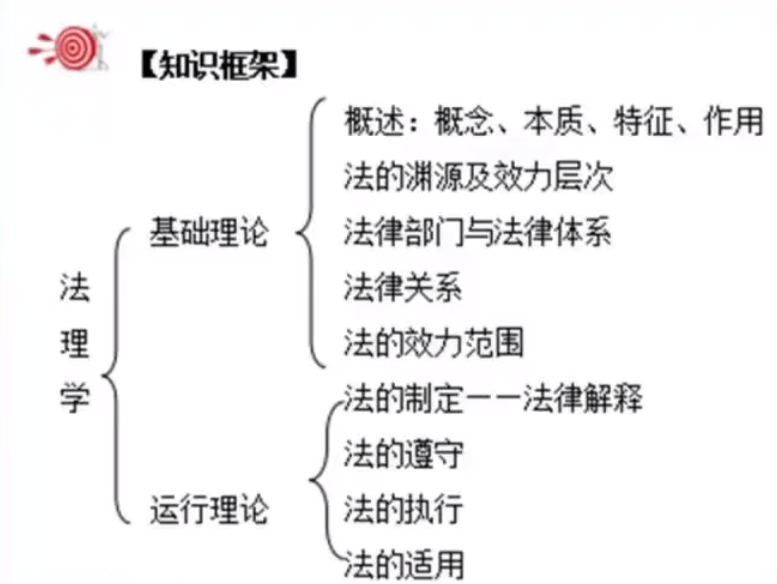
\includegraphics[scale=0.25]{law-theroy}\\ 
\end{frame}



%%%%%%%%%%%%%%%%%%%%%%%%%%%%%%%%%%%%%%%%
% A frame
%%%%%%%%%%%%%%%%%%%%%%%%%%%%%%%%%%%%%%%%
\begin{frame}[t]{法理学}

    真题:\\
    
\includegraphics[scale=0.3]{17-1}\\ 
\end{frame}

%%%%%%%%%%%%%%%%%%%%%%%%%%%%%%%%%%%%%%%%
% A frame
%%%%%%%%%%%%%%%%%%%%%%%%%%%%%%%%%%%%%%%%
\begin{frame}[t]{法理学}

    真题:\\
    
\includegraphics[scale=0.3]{17-1}\\ 
    答案:\textbf{B}\\
\end{frame}

%%%%%%%%%%%%%%%%%%%%%%%%%%%%%%%%%%%%%%%%
% A frame
%%%%%%%%%%%%%%%%%%%%%%%%%%%%%%%%%%%%%%%%
\begin{frame}[t]{法理学}
    滞后性\\
    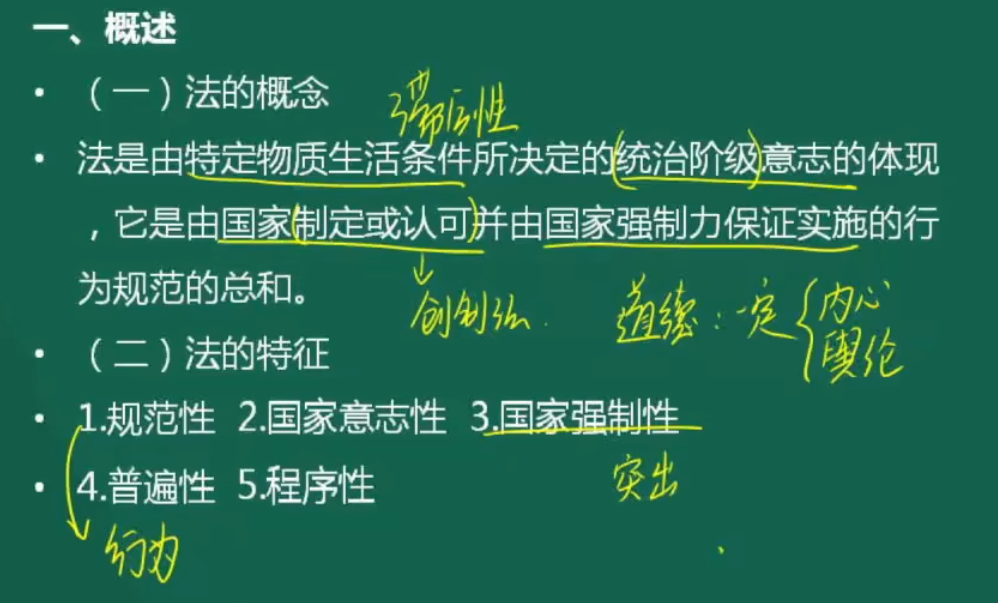
\includegraphics[scale=0.3]{law-intro}\\ 
    普遍性: 在我国内,1.法是普遍有效的, 2. 平等对待性\\
    程序性:法具有严格的程序\\
    \textbf{国家强制性}: 最突出的特征\\
\end{frame}

%%%%%%%%%%%%%%%%%%%%%%%%%%%%%%%%%%%%%%%%
% A frame
%%%%%%%%%%%%%%%%%%%%%%%%%%%%%%%%%%%%%%%%
\begin{frame}[t]{法理学}
    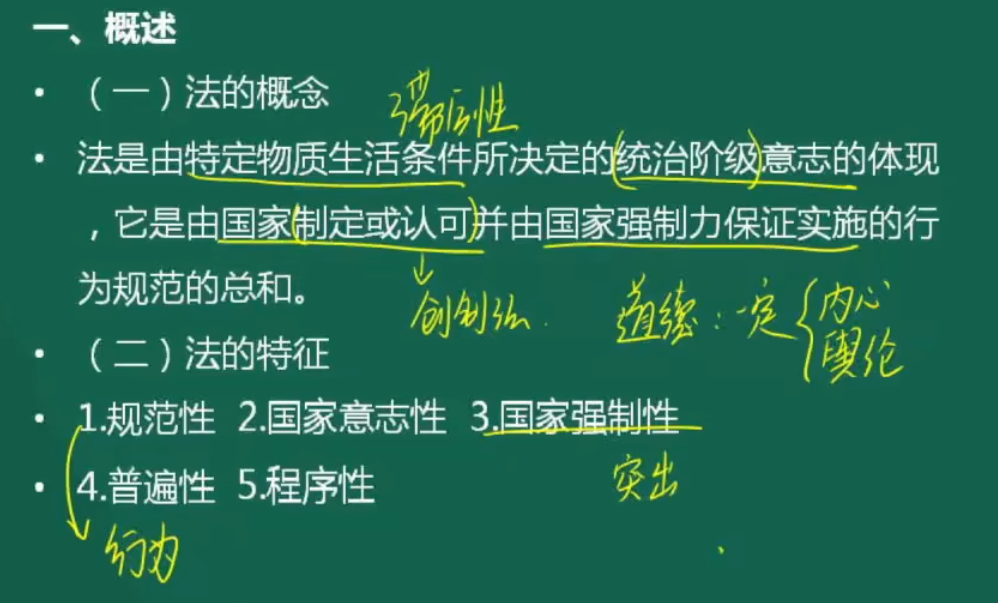
\includegraphics[scale=0.3]{law-intro}\\ 
    规范作用用来规范人\\
    社会作用: 对社会关系规范,1 维护统治阶级统治 2 维护社会稳定
\end{frame}


%%%%%%%%%%%%%%%%%%%%%%%%%%%%%%%%%%%%%%%%
% A frame
%%%%%%%%%%%%%%%%%%%%%%%%%%%%%%%%%%%%%%%%
\begin{frame}[t]{法理学}

    例子:\\
    孙杨 —— 无证驾驶 —— 横幅 ——  指引作用\\
    群众(评价作用) ——  孙杨 —— 无证驾驶 \\
    孙杨 —— 无证驾驶 —— 行政拘留 ——  法的强制作用\\
    孙杨 —— 无证驾驶 —— 报纸 ——  群众 ——  教育作用\\
    孙杨 ——   买车 ——  预测作用\\
\end{frame}

%%%%%%%%%%%%%%%%%%%%%%%%%%%%%%%%%%%%%%%%
% A frame
%%%%%%%%%%%%%%%%%%%%%%%%%%%%%%%%%%%%%%%%
\begin{frame}[t]{法理学}

    真题:\\
    
\includegraphics[scale=0.3]{001}\\ 
\end{frame}


%%%%%%%%%%%%%%%%%%%%%%%%%%%%%%%%%%%%%%%%
% A frame
%%%%%%%%%%%%%%%%%%%%%%%%%%%%%%%%%%%%%%%%
\begin{frame}[t]{法理学}

    真题:\\
    
\includegraphics[scale=0.3]{001}\\ 
    答案:\textbf{A,国家意志性}\\
\end{frame}



%%%%%%%%%%%%%%%%%%%%%%%%%%%%%%%%%%%%%%%%
% A frame
%%%%%%%%%%%%%%%%%%%%%%%%%%%%%%%%%%%%%%%%
\begin{frame}[t]{法理学}
    \textbf{区别:制定主体不同}\\
    
\includegraphics[scale=0.3]{law_scope}\\ 
    宪法 全国人大制定
    宪法(根本大法)修改:全国人大常务委员会\textbf{提议}/ 五分之一以上代表可以\textbf{提议}, 全体代表三分之二以上\textbf{通过}\\
    法律制定主体:1 全国人大(基本法) 2 全人常(其他法律)\\
    法律绝对保留四个方面: 刑 政 人 税\\
    行政法规:国务院, 自治法规:自治区/州/人大; 国际条例(认可而来的)
\end{frame}

%%%%%%%%%%%%%%%%%%%%%%%%%%%%%%%%%%%%%%%%
% A frame
%%%%%%%%%%%%%%%%%%%%%%%%%%%%%%%%%%%%%%%%
\begin{frame}[t]{法理学}
    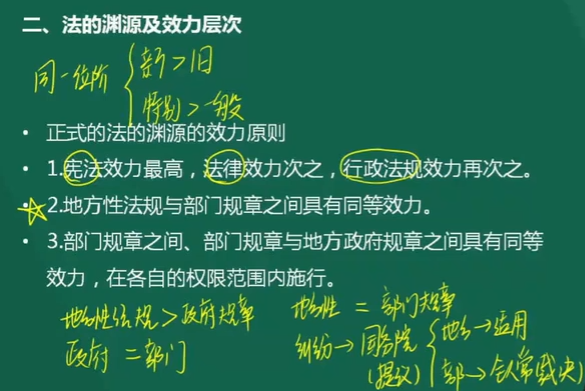
\includegraphics[scale=0.5]{law_priority}\\ 
    新法优于旧法,特别法优于一般法\\
\end{frame}

%%%%%%%%%%%%%%%%%%%%%%%%%%%%%%%%%%%%%%%%
% A frame
%%%%%%%%%%%%%%%%%%%%%%%%%%%%%%%%%%%%%%%%
\begin{frame}[t]{法理学}
    真题:\\
    
\includegraphics[scale=0.5]{002}\\ 
\end{frame}


%%%%%%%%%%%%%%%%%%%%%%%%%%%%%%%%%%%%%%%%
% A frame
%%%%%%%%%%%%%%%%%%%%%%%%%%%%%%%%%%%%%%%%
\begin{frame}[t]{法理学}
    真题:\\
    
\includegraphics[scale=0.5]{002}\\ 
    答案:\textbf{B,习惯}, 非正式渊源, (习惯, 判例,政策)\\
\end{frame}


%%%%%%%%%%%%%%%%%%%%%%%%%%%%%%%%%%%%%%%%
% A frame
%%%%%%%%%%%%%%%%%%%%%%%%%%%%%%%%%%%%%%%%
\begin{frame}[t]{法理学}
    
\includegraphics[scale=0.7]{lay_department}\\ 
\end{frame}

%%%%%%%%%%%%%%%%%%%%%%%%%%%%%%%%%%%%%%%%
% A frame
%%%%%%%%%%%%%%%%%%%%%%%%%%%%%%%%%%%%%%%%
\begin{frame}[t]{法理学}
    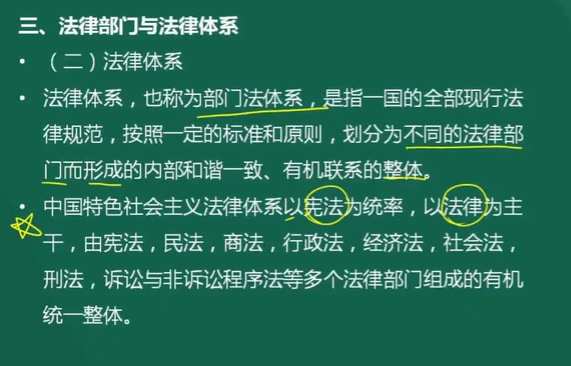
\includegraphics[scale=0.7]{law_arch}\\ 
\end{frame}

%%%%%%%%%%%%%%%%%%%%%%%%%%%%%%%%%%%%%%%%
% A frame
%%%%%%%%%%%%%%%%%%%%%%%%%%%%%%%%%%%%%%%%
\begin{frame}[t]{法理学}
    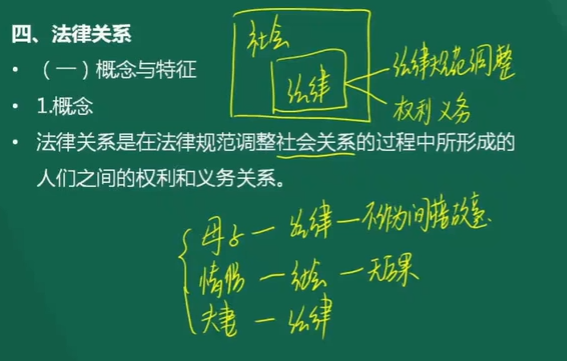
\includegraphics[scale=0.7]{law_relation}\\ 
\end{frame}



%%%%%%%%%%%%%%%%%%%%%%%%%%%%%%%%%%%%%%%%
% A frame
%%%%%%%%%%%%%%%%%%%%%%%%%%%%%%%%%%%%%%%%
\begin{frame}[t]{法理学}
    真题:\\
    
\includegraphics[scale=0.5]{003}\\ 
\end{frame}


%%%%%%%%%%%%%%%%%%%%%%%%%%%%%%%%%%%%%%%%
% A frame
%%%%%%%%%%%%%%%%%%%%%%%%%%%%%%%%%%%%%%%%
\begin{frame}[t]{法理学}
    真题:\\
    
\includegraphics[scale=0.5]{003}\\ 
    答案:\textbf{D,法律关系是以 主体,客体,内容,为三要素的社会关系}\\
\end{frame}



%%%%%%%%%%%%%%%%%%%%%%%%%%%%%%%%%%%%%%%%
% A frame
%%%%%%%%%%%%%%%%%%%%%%%%%%%%%%%%%%%%%%%%
\begin{frame}[t]{法理学}
    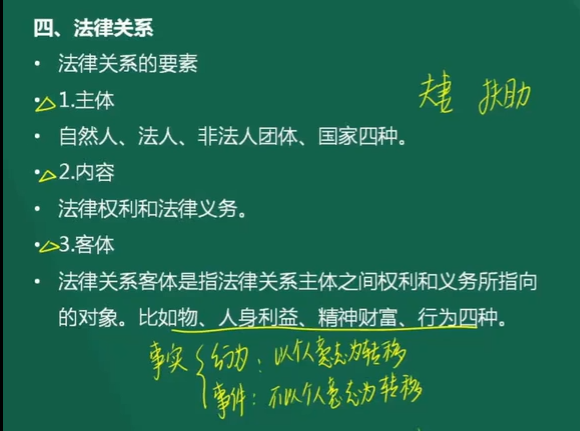
\includegraphics[scale=0.5]{law_element}\\ 
    法律行为以个人意志为转移\\
    法律事件不以个人意志为转移
\end{frame}

%%%%%%%%%%%%%%%%%%%%%%%%%%%%%%%%%%%%%%%%
% A frame
%%%%%%%%%%%%%%%%%%%%%%%%%%%%%%%%%%%%%%%%
\begin{frame}[t]{法理学}
    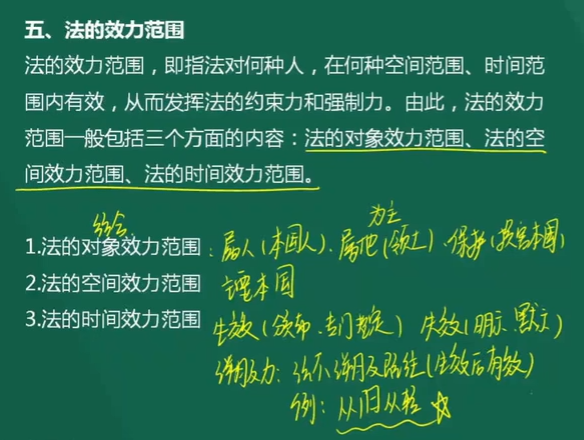
\includegraphics[scale=0.5]{law_range}\\ 
\end{frame}


%%%%%%%%%%%%%%%%%%%%%%%%%%%%%%%%%%%%%%%%
% A frame
%%%%%%%%%%%%%%%%%%%%%%%%%%%%%%%%%%%%%%%%
\begin{frame}[t]{法理学}
    
\includegraphics[scale=0.5]{law-run-theory}\\ 
\end{frame}

%%%%%%%%%%%%%%%%%%%%%%%%%%%%%%%%%%%%%%%%
% A frame
%%%%%%%%%%%%%%%%%%%%%%%%%%%%%%%%%%%%%%%%
\begin{frame}[t]{法理学}
    真题:\\
    
\includegraphics[scale=0.5]{004}\\ 
\end{frame}

%%%%%%%%%%%%%%%%%%%%%%%%%%%%%%%%%%%%%%%%
% A frame
%%%%%%%%%%%%%%%%%%%%%%%%%%%%%%%%%%%%%%%%
\begin{frame}[t]{法理学}
    真题:\\
    
\includegraphics[scale=0.5]{004}\\ 
    答案:\textbf{C,全国人大是立法机关, 进行立法解释}\\
司法机关——司法解释,国务院——行政解释,全国人大——立法解释,法律专家——非正式解释\\
\end{frame}

%%%%%%%%%%%%%%%%%%%%%%%%%%%%%%%%%%%%%%%%
% A frame
%%%%%%%%%%%%%%%%%%%%%%%%%%%%%%%%%%%%%%%%
\begin{frame}[t]{法理学}
    
\includegraphics[scale=0.5]{law-run-theory_2}\\ 
\end{frame}


\end{document}
